\section{Analysis}
\label{sec:analysis}

\subsection{Feasability of DNS request linking}
\fixme{rerun all experiments with more sites}
We perform 10-fold cross-validation for all of our experiments in the open
world setting. We monitor 10 sites with 100 instances each and
$10*100$ unmonitored sites.
Note that the ratio between monitored instances and unmonitored sites is 1:1,
ensuring that for the classifier there is equal probability in the testing
phase that a trace is a monitored or unmonitored site.
Furthermore, for all experiments we define an \emph{offset} that specifies
which sites on Alexa are monitored. An offset of 0 means that Alexa sites 1-10
are monitored and Alexa 11-1010 unmonitored. An offset of 10 means that
Alexa sites 11-20 are monitored, and Alexa 1-10 and 21-1010 unmonitored. We
never monitor an unmonitored site and vice versa. How popular monitored sites
are is a key factor in the effectiveness of our attacks.

Figure~\ref{fig:wfdns:torpct} shows the recall and precision for our WF+DNS
attacks as a function of the percentage of observed Tor exit bandwidth by the
attacker at offset $10^5$.
Recall measures the probability that a visit to a monitored page will
be detected, while precision measures the probability that a classification by
the classifier of a visit to a monitored site (positive test outcome) is the
correct one.

\begin{figure}[t]
\centering
\subfigure[Recall]{
	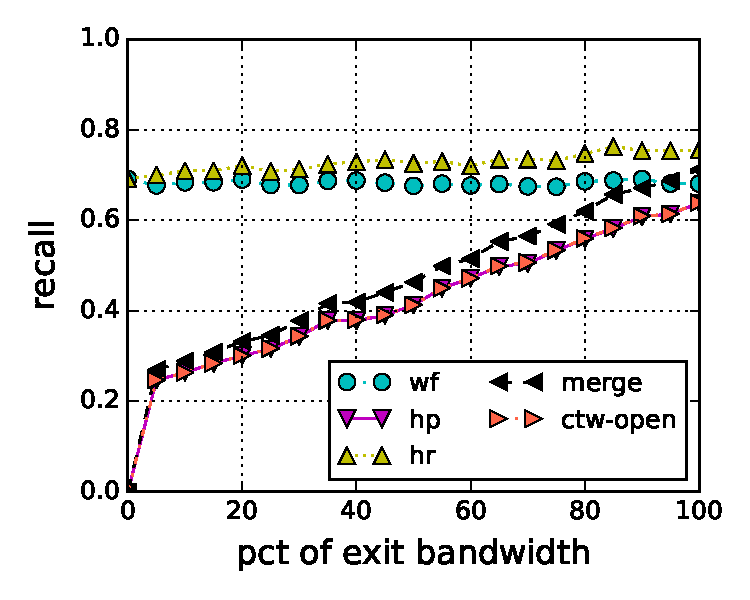
\includegraphics[width=0.466\linewidth]{figures/wfdns/10x100+1k-offset100k-recall}
    \label{fig:wfdns:torpct:recall}
}
\subfigure[Precision]{
	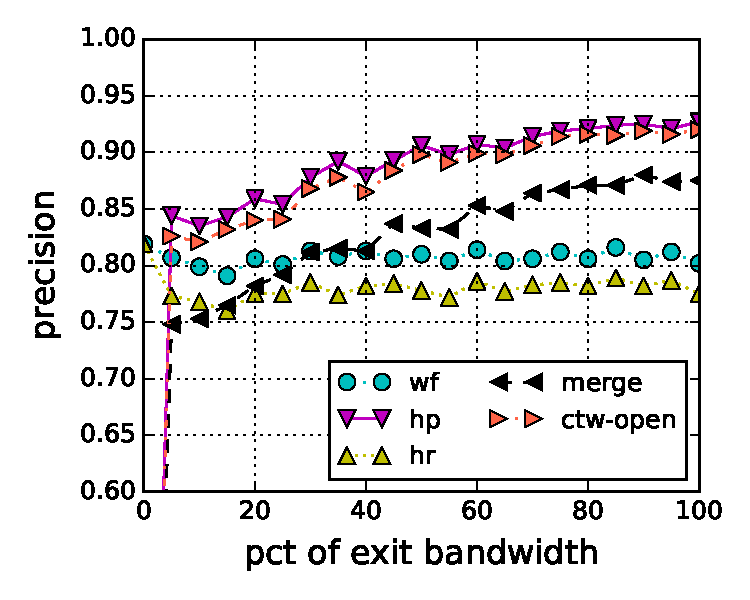
\includegraphics[width=0.466\linewidth]{figures/wfdns/10x100+1k-offset100k-precision}
    \label{fig:wfdns:torpct:precision}
}
\caption{10x100+1k-offset100k}
\label{fig:wfdns:torpct}
\end{figure}

% what to monitor is a key consideratio

% impact of:
% - fixing Tor TTL bug,
% - different min/max TTLs

% limitation: webSITES, not wePAGES in our analysis + what we get from DNS.

Figure~\ref{fig:wfdns:offsets} shows recall and precision at 100 percentage of
observed Tor exit bandwidth as a function of the offset.

\begin{figure}[t]
\centering
\subfigure[Recall]{
	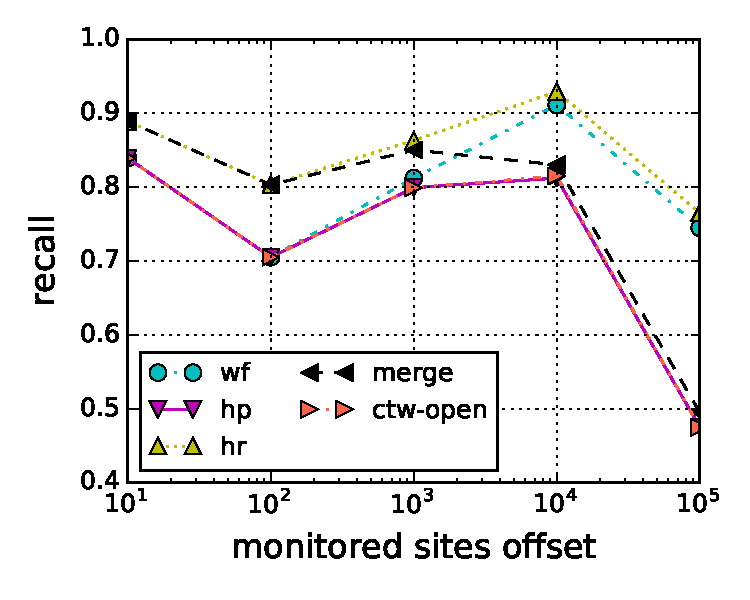
\includegraphics[width=0.466\linewidth]{figures/wfdns/10x100+1k-offsets-50pct-recall}
    \label{fig:wfdns:offsets:recall}
}
\subfigure[Precision]{
	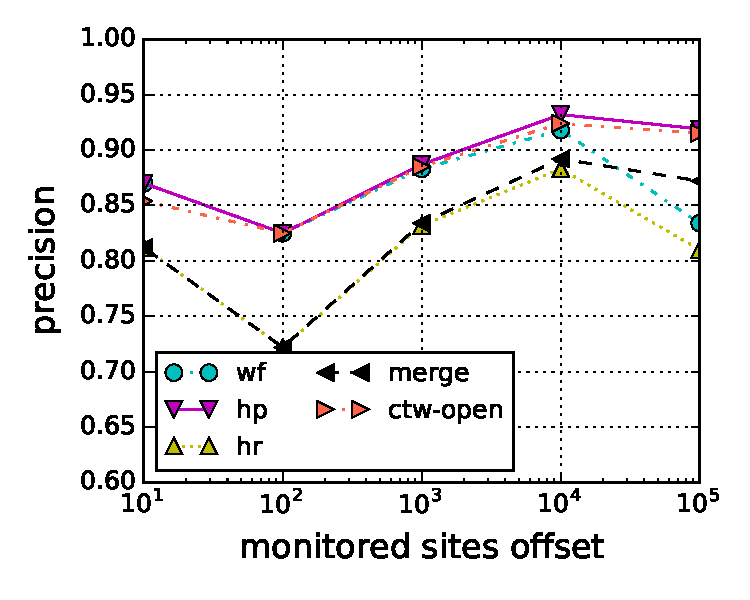
\includegraphics[width=0.466\linewidth]{figures/wfdns/10x100+1k-offsets-50pct-precision}
    \label{fig:wfdns:offsets:precision}
}
\caption{10x100+1k-offsets at 100 percentage of Tor exit bandwidth.}
\label{fig:wfdns:offsets}
\end{figure}

\fixme{ongoing work, considering dropping merge+hr since they seem useless
(trade recall for precision) and just complicate it all? As a bonus, we could
pick one more WF attack with the same approach and compare?}
